\lesson{Oct 11 2022}{Vectors}

\subsection{Formulation}
\label{sub:vector-formulation}

\begin{definition}[Vector]
    A mathematical object that has a:
    \begin{itemize}
        \item Magnitude
        \item Orientation
        \item Sense (sign)
    \end{itemize}
\end{definition}

We use arrows to represent vectors graphically, the choice of arrows is very similar to the choice of lengths to represent numbers.

\begin{definition}[Vector equality]
    For $\vec{a}$ to be equal to $\vec{b}$
    \begin{itemize}
        \item $|\vec{a}| = |\vec{b}|$
        \item $\vec{a} \parallel \vec{b}$
        \item Sense of $\vec{a}$ is the same as that of $\vec{b}$
    \end{itemize}
\end{definition}

The choice of such an equality, although looks natural, is a made construct. This specific equality is useful for our calculations. However, it is as real as $\frac{1}{2}=\frac{3}{6}$, which, even though represents the notion of ratios, is not \textit{real} since, clearly, the process of cutting a pizza into 2 pieces is different from cutting it into 6 piece.

\begin{note}
    Notice how the equality is defined in terms of the original definition.
\end{note}

\subsection{Arithmetic}%
\label{sub:vector-arithmetic}

\subsubsection{Addition}%
\label{ssub:vector-addition}

\begin{definition}[Vector addition]
        Vector $\vec{a}+\vec{b}$ starts at the end of $\vec{A}$ and ends at the end of $\vec{B}$
\end{definition}

\begin{figure}[H]
    \begin{center}
        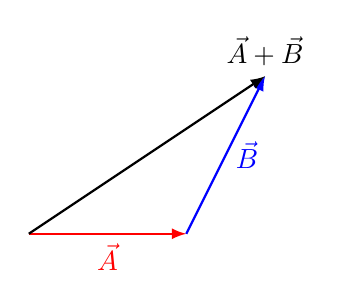
\begin{tikzpicture}[scale=1, transform shape]
            \draw[red,thick,-{latex}] (0,0) -- (2,0) node[midway, below]
                {$\vec{A}$};
            \draw[blue,thick,-{latex}] (2,0) -- (3,2) node[midway, right]
                {$\vec{B}$};
            \draw[thick,-{latex}] (0,0) -- (3,2) node[above]
                {$\vec{A}+\vec{B}$};
            % \draw[thick,dashed,->] (2,0) -- (3,2) node[right] {$\vec{B}$};
            % \draw[thick,dashed,->] (1,2) -- (3,2) node[above] {$\vec{A}$};
        \end{tikzpicture}
    \end{center}
    \caption{Sum of two vectors}%
    \label{fig:vector-sum}
\end{figure}


This definition is based on the practicality of such a geometrical construct according to real life observations. Moreover, this enables commutative and associative.

\begin{figure}[htpb]
    \begin{center}
        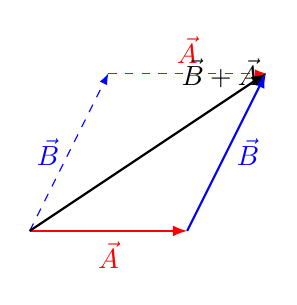
\begin{tikzpicture}[scale=1, transform shape]
            \draw[red,thick,-{latex}] (0,0) -- (2,0) node[midway, below] {$\vec{A}$};
            \draw[blue,thick,-{latex}] (2,0) -- (3,2) node[midway, right] {$\vec{B}$};
            \draw[red,dashed,-{latex}] (1,2) -- (3,2) node[midway, above] {$\vec{A}$};
            \draw[blue,dashed,-{latex}] (0,0) -- (1,2) node[midway, left] {$\vec{B}$};
            \draw[thick,-{latex}] (0,0) -- (3,2) node[above, left=-1.1] {$\vec{B}+\vec{A}$};
        \end{tikzpicture}
    \end{center}
    \caption{Commutative property of vector sum}%
    \label{fig:vector-sum-com}
\end{figure}

\begin{figure}[htpb]
    \begin{center}
        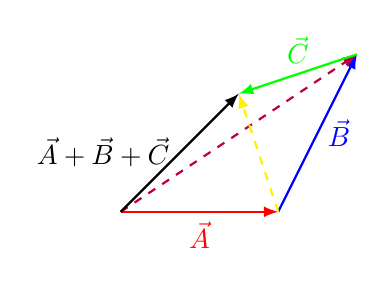
\begin{tikzpicture}[scale=1, transform shape]
            \draw[red,thick,-{latex}] (0,0) -- (2,0) node[midway, below] {$\vec{A}$};
            \draw[blue,thick,-{latex}] (2,0) -- (3,2) node[midway, right] {$\vec{B}$};
            \draw[dashed,purple,thick,-{latex}] (0,0) -- (3,2);
            \draw[green,thick,-{latex}] (3,2) -- (1.5,1.5) node[midway, above] {$\vec{C}$};
            \draw[dashed,yellow,thick,-{latex}] (2,0) -- (1.5,1.5);
            \draw[thick,-{latex}] (0,0) -- (1.5,1.5) node[midway, left] {$\vec{A}+\vec{B}+\vec{C}$};
        \end{tikzpicture}
    \end{center}
    \caption{Associative property of vector sum}%
    \label{fig:vector-sum-com}
\end{figure}

We define the zero vector due to the usefulness of zero in normal arithmetic.

\begin{definition}[Zero Vector]
    \[
        \vec{v}+\vec{0}=\vec{v}
    .\] 
\end{definition}

\begin{note}
    \begin{align*}
        \vec{0} & \neq 0. \\
        |\vec{0}| & = 0.
    \end{align*}
\end{note}

\subsection{Cartesian coordinates}%
\label{sub:cartesian}

\change{Add operations before this}

To use vectors in a more practical context, we put them onto the Cartesian coordinates where:
\begin{itemize}
    \item All vectors starts from the origin point of the coordinate system we chose.
    \item The tip of the vector lies inside the coordinate space we chose.
\end{itemize}

It is not physically helpful to use vectors starting from different origin points, and when this is needed, it helps to clarify the difference between various systems for calculations to be accurate.

In order to actually use the proprieties of the Cartesian coordinate, we have to associate the vector's tip with some point $(a,b)$. Sometimes vectors and points are used interchangeably. Whenever they are used in such manner, the physical context clarifies this confusion, but in some cases, they both are used within the same system where the distinction between them is needed.

\begin{note}
    Vectors are not points, neither are equivalent to them.
\end{note}

\subsubsection{Unit vectors}%
\label{ssub:unit-vectors}


To both avoid the confusion with points and make calculations more computable we use unit vectors. Unite vectors are like a reference point for a given system. Their physical value is completely arbitrary, although usually used with real life units (meter, km, mile, etc).

\begin{definition}[Unit vectors]
    Vectors of length 1, orthogonal to each other, and parallel to the axes of the coordinate system, such that:
    \begin{itemize}
        \item the tip of $e_1$ is on the point $(1,0,\ldots)$.
        \item the tip of $e_2$ is on the point $(0,1,\ldots)$.
            \\ \vdots
        \item the tip of $e_n$ is on the point $(0,0,\ldots,1)$.
    \end{itemize}
\end{definition}

We usually refer to the first unit vectors as:
\begin{itemize}
    \item $e_1 = \hat{i}$
    \item $e_2 = \hat{j}$
    \item $e_3 = \hat{k}$
\end{itemize}

$\hat{i}$ and $\hat{j}$ forms the relation $\vec{A}=a\hat{i}+b\hat{j}$.

% - Here, we define scalar multiplication and unit vectors.
% - ==NOTE:== vectors **are not** points
% - Although they are similar mathematical objects, their definitions are vastly different, so whenever they are used in the same context the difference need to be clarified.
% - The notation may be used interchangeably if the physical context does not need differentiation between them.

% \begin{theorem}
% This is a theorem.
% \end{theorem}
% \begin{proof}
% This is a proof.
% \end{proof}
% \begin{example}
% This is an example.
% \end{example}
% \begin{explanation}
% This is an explanation.
% \end{explanation}
% \begin{claim}
% This is a claim.
% \end{claim}
% \begin{corollary}
% This is a corollary.
% \end{corollary}
% \begin{prop}
% This is a proposition.
% \end{prop}
% \begin{lemma}
% This is a lemma.
% \end{lemma}
% \begin{question}
% This is a question.
% \end{question}
% \begin{solution}
% This is a solution.
% \end{solution}
% \begin{exercise}
% This is an exercise.
% \end{exercise}
% \begin{definition}[Definition]
% This is a definition.
% \end{definition}
% \begin{note}
% This is a note.
% \end{note}

% subsection sub_section_2 (end)

\newpage
